\documentclass[11pt, titlepage]{article}

\usepackage[letterpaper, hmargin=1in, bmargin=1in, tmargin=1.3in,
headheight=26pt]{geometry}

\usepackage{graphicx}
\usepackage{booktabs}
\usepackage{longtable}
\usepackage{tabularx}
\usepackage[breaklinks=true]{hyperref}
\usepackage{array}   % Used for table formatting
\newcolumntype{P}[1]{>{\raggedright\let\newline\\\arraybackslash\hspace{0pt}}m{#1}}
\newcolumntype{C}[1]{>{\centering\arraybackslash}m{#1}}
\newcolumntype{N}[1]{>{\centering\arraybackslash}p{#1}}
\usepackage{multirow}
\usepackage[shortcuts]{extdash}
\usepackage[usenames,dvipsnames,table]{xcolor}
\usepackage{url}

\usepackage[nottoc,notlof,notlot,numbib]{tocbibind}

\usepackage{natbib}

\usepackage[page]{totalcount}

\usepackage{fancyhdr}
\fancyhf{}
\lhead{Master Test Plan \\ \progname{}}
\rhead{Geneva M. Smith \\ Dept. of Computing and Software---McMaster University}
\lfoot{Ver.~\ref{current_version_TestPlan}}
\rfoot{\thepage\ of \thepages}

\renewcommand{\footrule}{\vbox to 0pt
    {\makebox[\textwidth]{\hrulefill}\vss}}

\newcommand{\colourRow}{\rowcolor[gray]{0.9}}
\newcommand{\colourCell}{\cellcolor[gray]{0.9}}

\definecolor{CoolPurple}{RGB}{117, 0, 235}
\definecolor{NatureGreen}{RGB}{8, 104, 11}
\definecolor{SeaBlue}{RGB}{6, 97, 122}
\definecolor{Lilac}{RGB}{178, 131, 206}

\hypersetup{
    bookmarks=true,
    colorlinks=true,
    linktoc=all,
    linkcolor=CoolPurple,
    citecolor=NatureGreen,
    filecolor=WildStrawberry,
    urlcolor=SeaBlue
}

\newcommand{\citepg}[2]{\citeauthor{#1}, \citeyear{#1}, p.~#2}
\newcommand{\citeg}[1]{\citeauthor{#1}, \citeyear{#1}}

\makeatletter
\newcommand\newref[1]{#1\def\@currentlabel{#1}}
\makeatother

%% Comments

\usepackage{color}

\newif\ifcomments\commentstrue

\ifcomments
\newcommand{\authornote}[3]{\textcolor{#1}{[#3 ---#2]}}
\newcommand{\todo}[1]{\textcolor{red}{[TODO: #1]}}
\else
\newcommand{\authornote}[3]{}
\newcommand{\todo}[1]{}
\fi

\newcommand{\wss}[1]{\authornote{blue}{SS}{#1}}
\newcommand{\wgs}[1]{\authornote{teal}{GS}{#1}}
\newcommand{\wjc}[1]{\authornote{purple}{JC}{#1}}

\newcommand{\progname}{EMgine} % PUT YOUR PROGRAM NAME HERE

\newcommand{\conceptVersion}{1.0}
\newcommand{\srsVersion}{1.5.1}
\newcommand{\mgversion}{1.5}
\newcommand{\misversion}{0.1.1}
\newcommand{\codeversion}{0.1}
\newcommand{\mastertestplanVersion}{1.0}
\newcommand{\verifytestplanVersion}{1.0}
\newcommand{\validatetestplanVersion}{1.0}
\newcommand{\manualversion}{?}

\newcommand{\timetype}{\mathbb{T}}
\newcommand{\deltatimetype}{\mathbb{T}_{\Delta}}
\newcommand{\energytype}{\mathbb{J}}
\newcommand{\energychangetype}{\mathbb{J}_{\Delta}}
\newcommand{\stringtype}{\text{String}}
\newcommand{\emotionintensitytype}{\mathbb{I}}
\newcommand{\responsestrength}{\mathbb{I}_{\Delta}}
\newcommand{\emotionstatetype}{\mathbb{ES}}
\newcommand{\emotionstatedecaytype}{\mathbb{ES}_\lambda}
\newcommand{\emotiontype}{\mathbb{E}}
\newcommand{\emotionkindstype}{\mathbb{K}}
\newcommand{\emotionequilibriumtype}{\mathbb{ES_{\rightleftharpoons}}}
\newcommand{\emotiondecaytype}{\mathbb{I_{\lambda}}}
\newcommand{\egotype}{\mathbb{O}}
\newcommand{\egoidentitytype}{\mathbb{ID}}
\newcommand{\goaltype}{\mathbb{G}}
\newcommand{\plantype}{\mathbb{P}}
\newcommand{\padpoint}{P_{\left(P,A,D\right)}}
\newcommand{\goallabeltype}{\mathbb{L}}
\newcommand{\worldtype}{\mathbb{W}}
\newcommand{\worldstatetype}{\mathbb{S}}
\newcommand{\worldstatechangetype}{\mathbb{S}_{\Delta}}
\newcommand{\statedistancetype}{\mathbb{D}}
\newcommand{\statedistancechangetype}{\mathbb{D}_{\Delta}}
\newcommand{\indexsettype}{\mathbb{IS}}
\newcommand{\goalegotype}{\mathbb{GE}}
\newcommand{\socialrelationtype}{{R^{S}}}
\newcommand{\socialattachmenttype}{\mathbb{SA}}
\newcommand{\actiontype}{\mathbb{AC}}
\newcommand{\actortype}{\mathbb{A}}
\newcommand{\attentiontype}{\mathbb{AT}_x}
\newcommand{\probabilitytype}{\left[0,1\right]}
\newcommand{\maxval}{\mathsf{MAX}}
\newcommand{\True}{\mathit{True}}
\newcommand{\False}{\mathit{False}}
\newcommand{\defEq}{\text{ } \mathlarger{\mathlarger\circeq} \text{ }}

\newcommand{\mOtherChange}{\mathit{otherChange}}
\newcommand{\mActor}{\mathit{actor}}
\newcommand{\mDeliberate}{\mathit{deliberate}}
\newcommand{\mImportance}{\mathit{importance}}
\newcommand{\mFear}{\mathtt{Fear}}
\newcommand{\mAnger}{\mathtt{Anger}}
\newcommand{\mSadness}{\mathtt{Sadness}}
\newcommand{\mJoy}{\mathtt{Joy}}
\newcommand{\mInterest}{\mathtt{Interest}}
\newcommand{\mSurprise}{\mathtt{Surprise}}
\newcommand{\mDisgust}{\mathtt{Disgust}}
\newcommand{\mTrust}{\mathtt{Acceptance}}
\newcommand{\mStore}{\mathit{Store}}
\newcommand{\mControl}{\mathit{Control}}
\newcommand{\mGenerate}{\mathit{Generate}}
\newcommand{\mDecay}{\mathit{Decay}}
\newcommand{\mAppraisal}{\mathit{Appraisal}}

\usepackage[shortlabels, inline]{enumitem}

\begin{document}

    \newcounter{pages}
    \setcounter{pages}{\totalpages}

    \begin{titlepage}
        \thispagestyle{empty}

        \title{Master Test Plan for \progname{}: A Computational Model of
        Emotion for Enhancing Non-Player Character Believability in Games}
        \author{Geneva M. Smith}
        \date{Version~\ref{current_version_TestPlan} (March 24, 2023)}

        \maketitle
    \end{titlepage}

    \pagestyle{fancy}

    \vspace*{\fill}
    \section*{Revision History}
    \begin{center}
        \begin{tabular}{m{0.17\linewidth}C{0.13\linewidth}m{0.6\linewidth}}
            \toprule {\bf Date} & {\bf Version} & {\bf Notes}\\
            \midrule
            \vspace*{1mm}March 24, 2023 &
            \vspace*{1mm}\newref{1.0}\label{current_version_TestPlan} &
            \vspace*{5mm}
            \begin{itemize}[noitemsep, nosep]
                \item Initial version
            \end{itemize} \\
            \bottomrule
        \end{tabular}
    \end{center}
    \vspace*{\fill}

    \clearpage

    \tableofcontents

    \clearpage

    \listoftables

    \listoffigures

    \clearpage

    \section{Symbols, Abbreviations and Acronyms}\label{sec:refs}
For \progname{}'s other symbols, abbreviations, and acronyms, see the:
\begin{itemize}
    \item Software Requirement Specification (SRS) at
    \href{https://github.com/GenevaS/EMgine/blob/main/docs/SRS/EMgine_SRS.pdf}{https://github.com/GenevaS/EMgine/blob/
        \newline main/docs/SRS/EMgine\_SRS.pdf}, and
    \item Module Guide (MG) at
    \href{https://github.com/GenevaS/EMgine/blob/main/docs/Design/MG/EMgine_MG.pdf}{https://github.com/GenevaS/EMgine/blob/main/docs/Design/\newline
        MG/EMgine\_MG.pdf}, and
    \item Module Interface Specification (MIS) at
    \href{https://github.com/GenevaS/EMgine/blob/main/docs/Design/MIS/EMgine_MIS.pdf}{https://github.com/GenevaS/EMgine/blob/main/
        \newline docs/Design/MIS/EMgine\_MIS.pdf}.
\end{itemize}

\begin{center}

    \renewcommand{\arraystretch}{1.2}
    \begin{tabular}{c l}
        \toprule
        \textbf{Abbrv.} & \textbf{Description} \\

        \midrule

        \colourRow ATP & Acceptance Test Plan \\

        CME & Computational Model of Emotion \\

        %CS & Computer Science \\

        %\colourRowHCI & Human-Computer Interaction \\

        \colourRow IDE & Integrated Development Environment \\

        M & Module defined in the MG \\

        \colourRow MG & Module Guide \\

        MIS & Module Interface Specification \\

        \colourRow MTP & Master Test Plan \\

        NF & Nonfunctional Requirement defined in the SRS \\

        \colourRow NPC & Non-Player Character (Video Games) \\

        R & Functional Requirement defined in the SRS \\

        \colourRow SDA & Software Development Artifact \\

        %SE & Software Engineering \\

        SIUTP & System, Integration, and Unit Test Plan \\

        \colourRow SDLC & Software Development Life Cycle \\

        SRS & Software Requirements Specification \\

        \colourRow T & Test\\

        V \& V & Verification and Validation \\

        \colourRow VS & Microsoft Visual Studio \\

        \bottomrule

    \end{tabular}

\end{center}

    \clearpage

    \section{Introduction}
This document describes the System, Integration, and Unit Test Plan (SIUTP) for
\progname{}. Its purpose is to describe the testing efforts to verify the
ability of \progname{}'s implementation to meet its functional and
nonfunctional requirements as described in its Software Requirements
Specification (SRS, Version~\srsVersion) and additional data types and models
as described in its Module Guide (MG, Version~\mgversion) and Module Interface
Specification (MIS, Version~\misversion). This also acts as a basis for
regression testing as \progname{} is developed further. It describes tests for
each requirement and module, traceability between tests and \progname{}'s
requirements, and testing and verification tools.

This test plan does \textit{not} include validation efforts to evaluate
\progname{}'s acceptability for its end-users and stakeholders. That
information is in its Acceptance Test Plan (ATP).

The document's content and organization is loosely based on IEEE Std 829-2008
Clause 9: Level Test Plan (LTP)~\citep{vvDocIEEE}.

\subsection{Summary of \progname{}'s Purpose and Design Goals}
\progname{} is a Computational Model of Emotion (CME) for Non-Player Characters
(NPCs) to enhance their believability, with the goal of improving long-term
player engagement. \progname{} is for \textit{emotion generation}, accepting
user-defined information from a game environment to determines what emotion and
intensity a NPC is ``experiencing''. How the emotion is expressed and what
other effects it could have on game entities is left for game
designers/developers to decide.

\progname{} aims to provide a feasible and easy-to-use method for game
designers/developers to include emotion in their NPCs, they perceive to be
challenging with the current tools and
restrictions~\citep{broekens2016emotional}. \progname{} should be modular and
portable such that game designers/developers can use it in their regular
development environment, and should not require knowledge of affective science,
psychology, and/or emotion theories. Therefore, it is a library of components
to maximize a game designer/developer's control over how and when \progname{}
functions.

\subsection{Scope of Testing Efforts}
The overall goals of \progname{}'s system, integration, and unit testing effort
are:
\begin{enumerate}

    \item Ensure traceability between \progname{}'s verification efforts and
    its SRS, MG, and MIS

    \item Build confidence in the correctness and accuracy of \progname{}'s
    source code

    \item Build confidence in \progname{}'s overall verification efforts

\end{enumerate}

This test plan must be \textit{reviewed} for each new major version of
\progname{}'s SRS, MG, and/or MIS and revised accordingly. This ensures that
these testing efforts remain relevant throughout \progname{}'s development. For
new minor versions of \progname{}'s SRS, MG, and/or MIS, the review can be
limited to only those sections related to SRS, MG, and/or MIS modifications to
help reduce the effort required when testing the next major version.

This test plan must be \textit{executed} in full for each new major version of
\progname{}'s source code. Previous versions do not need to be retested. The
SIUTP can be partially executed for new minor versions of the source code to
help reduce the effort required when testing the next major version.

The SIUTP describes the ``Dynamic Testing Method'' for Implementation
Verification referenced in \progname{}'s Master Test Plan (MTP)
Section~\ref{plan:implementation}.

\subsection{Project Organization}
\progname{}'s development uses the general software development life cycle
processes of requirements analysis, architecture and design definition,
implementation, verification, and validation. Each of these processes outputs at
least one Software Development Artifact (SDA) which serves as a description of
the process's results and becomes an input to subsequent processes
(Figure~\ref{fig:dependencies}). Each SDA has an associated verification and/or
validation plan (Table~\ref{tab:verificationPlanLocation}) to ensure that it
adheres to the \progname{}'s concept.

\vspace*{\fill}
\begin{figure}[!h]
    \centering
    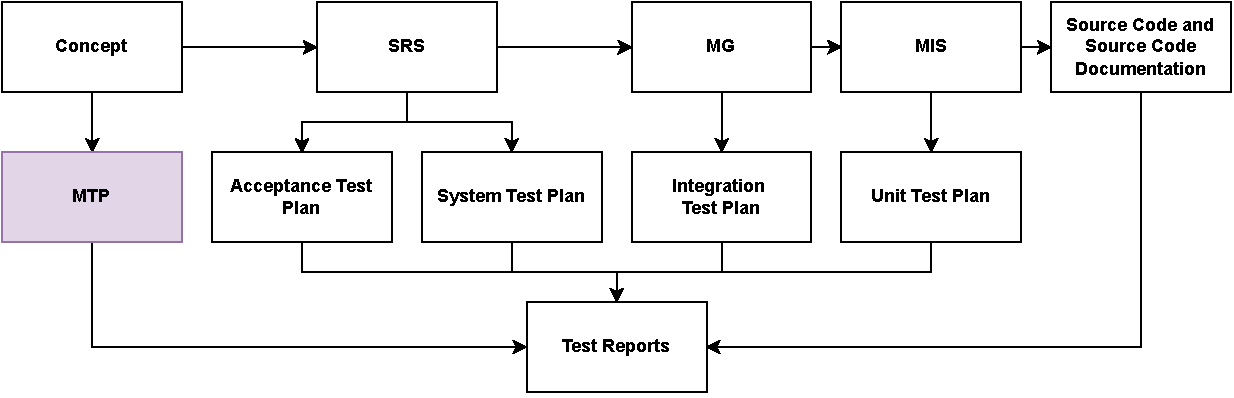
\includegraphics[width=\textwidth]{figures/mtpOrg.pdf}
    \caption{Dependencies Between \progname{}'s SDAs (MTP Highlighted)}
    \label{fig:dependencies}
\end{figure}

\begin{table}[!h]
    \renewcommand{\arraystretch}{1.2}
    \centering
    \caption{Location of V \& V Plans for \progname{}'s SDAs}
    \label{tab:verificationPlanLocation}
    \begin{tabular}{P{0.38\linewidth}P{0.5\linewidth}}
        \toprule
        \textbf{SDA} & \textbf{Location of V \& V Plan} \\

        \midrule

        \colourRow Concept Summary & -- \\

        Master Test Plan & Master Test Plan \\

        \colourRow Software Requirements Specification & Master Test Plan \\

        Module Guide & Master Test Plan \\

        \colourRow Module Interface Specification & Master Test Plan \\

        System, Integration, and Unit Test Plan & Master Test Plan \\

        \colourRow Acceptance Test Plan & Master Test Plan \\

        Source Code and Source Code Documentation& System, Integration, and
        Unit Test Plan \newline Acceptance Test Plan \\

        \bottomrule
    \end{tabular}
\end{table}
\vspace*{\fill}

\subsection{Relevant Documentation}
The Master Test Plan (MTP) refers to the following Software Development
Artifacts (SDAs):
\begin{itemize}

    \item \textbf{Title}: Concept Summary for \progname{}: A Computational
    Model of Emotion for Enhancing Non-Player Character Believability in Games
    \\
    \textbf{Location}:
    \href{https://github.com/GenevaS/EMgine/blob/main/docs/ConceptSummary/EMgine_ConceptSummary.pdf}{https://github.com/GenevaS/EMgine/blob/main/docs/ConceptSummary/\newline
     EMgine\_ConceptSummary.pdf} \\
    \textbf{Description}: Product of the concept definition process. An
    overview of \progname{} purpose, design goals, and motivation.

    \item \textbf{Title}: Software Requirements Specification for \progname{}:
    A Computational Model of Emotion for Enhancing Non-Player Character
    Believability in Games \\
    \textbf{Location}:
    \href{https://github.com/GenevaS/EMgine/blob/main/docs/SRS/EMgine_SRS.pdf}{https://github.com/GenevaS/EMgine/blob/main/docs/SRS/EMgine\_SRS.pdf}
     \\
    \textbf{Description}: Product of the requirements analysis process.
    \progname{}'s problem domain, purpose, underlying models, requirements
    (functional and nonfunctional), and likely changes.

    \item \textbf{Title}: Module Guide for \progname{}: A Computational Model
    of Emotion for Enhancing Non-Player Character Believability in Games \\
    \textbf{Location}:
    \href{https://github.com/GenevaS/EMgine/blob/main/docs/Design/MG/EMgine_MG.pdf}{https://github.com/GenevaS/EMgine/blob/main/docs/Design/MG/\newline
     EMgine\_MG.pdf} \\
    \textbf{Description}: Product of the architecture definition process. An
    overview of \progname{}'s architecture and component modules.

    \item \textbf{Title}: Module Interface Specification for \progname{}: A
    Computational Model of Emotion for Enhancing Non-Player Character
    Believability in Games \\
    \textbf{Location}: TDB \\
    \textbf{Description}: Product of the design definition process.
    Specifications of each module in \progname{} such that they are readily
    implementable.

    \item \textbf{Title}: Source Code and Documentation for \progname{}: A
    Computational Model of Emotion for Enhancing Non-Player Character
    Believability in Games \\
    \textbf{Location}: TDB \\
    \textbf{Description}: Product of the implementation process. A
    software-based realization of \progname{}'s requirements and design,
    accompanied by documentation of the resulting components and/or processes.

    \item \textbf{Title}: User Manual for \progname{}: A Computational Model
    of Emotion for Enhancing Non-Player Character Believability in Games \\
    \textbf{Location}: TDB \\
    \textbf{Description}: Product of the implementation process. A document
    written for \progname{}'s users to help them learn about and use
    \progname{}.

\end{itemize}

\noindent \progname{} has additional test plan documents as follows:
\begin{itemize}

    \item \textbf{Title}: System, Integration, and Unit Test Plan for
    \progname{}: A Computational Model of Emotion for Enhancing Non-Player
    Character Believability in Games \\
    \textbf{Location}: TDB \\
    \textbf{Description}: Test specifications to evaluate \progname{}'s models
    with respect to its design specifications (see
    Section~\ref{plan:implementation}).

    \clearpage\item \textbf{Title}: Acceptance Test Plan for \progname{}: A
    Computational Model of Emotion for Enhancing Non-Player Character
    Believability in Games \\
    \textbf{Location}: TDB \\
    \textbf{Description}: Test specifications to evaluate the ability of
    \progname{}'s models to produce expected emotions and intensities (see
    Section~\ref{plan:validate}).

\end{itemize}

\noindent This document also refers to the:
\begin{itemize}

    \item IEEE Standard for Software and System Test Documentation (IEEE
    Std 829-2008)~\citep{vvDocIEEE} to inform the creation of this document,
    the System, Integration, and Unit Test Plan, and the Acceptance Test Plan

    \item IEEE Standard for System, Software, and Hardware Verification and
    Validation (IEEE Std 1012-2016)~\citep{vvIEEE} to inform the creation of
    this document and the System, Integration, and Unit Test Plan

    \item IEEE Recommended Practice for Software Requirements Specifications
    (IEEE Std 830-1998 (R2009))~\citep{srsIEEE} to inform the evaluation of
    \progname{}'s Software Requirements Specification (SRS)

    \item ISO/IEC/IEEE International Standard - Systems and software
    engineering -- System life cycle processes (ISO/IEC/IEEE
    15288:2015(E))~\citep{slcIEEE} to inform the evaluation of \progname{}'s
    design

\end{itemize}

\subsection{Testing and Verification Tools}\label{sec:tools}
\progname{}'s development uses the C\# programming language because it is one
of the languages supported in Unity, a well-known game development
platform~\citep{unity3Dcsharp}. The supporting Integrated Development
Environment (IDE), Microsoft Visual Studio (VS), is the default script editor
in Unity. \progname{} development uses VS 2022 (Community Edition), which can
access the following tools:
\begin{itemize}

    \item \textbf{NUnit Unit Testing Framework} \\
    This supports the bulk of the automated testing approach for unit,
    integration, system, and regression testing. The IDE is configured to
    automatically run existing unit tests when it is compiling the code base.
    Unity Testing Framework uses custom integration of NUnit
    3.5~\citep{unity3Dtestingfw}.

    \item \textbf{Moq Library for .NET} \\
    This supports tests that rely on components that do not have a concrete
    implementation, such as the user-defined data types
    %(Section~\ref{sec_sysUserDataTypes}).
    It allows the definition of mocked
    interface calls within unit tests that are type-safe~\citep{moq}.

    \item \textbf{Performance Analysis} \\
    \progname{} uses the performance tools built into VS 2022, which includes
    CPU, memory, and time usage tools~\citep{vs2022perf}.

    \item \textbf{Code Style and Quality Analyzers} \\
    \progname{}'s development uses the official .NET Compiler Platform
    (Roslyn)~\citep{roslyn} and the third-party Roslynator~\citep{roslynator}
    analyzers to help adhere to good code quality and style practices. The
    Unity documentation also references Roslyn analyzers for code style and
    quality~\citep{unity3Droslyn}.

\end{itemize}

    \clearpage

    \section{Details of the Master Test Plan}\label{testplan_highlevel}
This section outlines the methodologies and tools for Verification and
Validation (V \& V), and the team responsible for executing the plan for each
of \progname{}'s Software Development Artifacts (SDAs).

\subsection{Test Plan Verification}\label{sec:mtpVV}
The goal of Test Plan verification is to evaluate all test plan documents for
correctness, consistency, completeness, readability, feasibility, and
traceability.

\paragraph{Method} The test plan verification plan relies on peer
review/document inspection with the following stages:
\begin{enumerate}

    \item Preparation: Participants review the test plan documents with respect
    to their assigned role and goals (Table~\ref{tab:rolesTestPlan})

    \item Meeting: Participants meet to discuss findings, potential issues, and
    proposed action plans to address them

    \item Rework: The test plan author(s) revise the document(s) to address
    raised issues, guided by the proposed action plans

    \item Follow Up: Participants verify that raised issues have been addressed
    satisfactorily

\end{enumerate}

A recording device might be used to capture meeting proceedings in place of
physical note taking so that all participants can focus on the discussion.

Peer review/inspection begins when there is a new major version of a test plan
document. Peer review/inspection need be done on those documents only.

Peer review/inspection ends when reviewers agree that there are no issues that
will likely result in the inability to execute any element of the plans and
verify that all plan components contribute to \progname{}'s overall
verification and validation (V \& V).

\paragraph{Roles and Responsibilities} To assist in the achievement of their
assigned goals (Table~\ref{tab:rolesTestPlan}) using peer review/document
inspection:
\begin{itemize}

    \item Primary team members are responsible for ensuring that reviewers have
    the necessary materials, moderating the inspection process and reading
    through the test plan document(s) during the meeting

    \item Secondary and tertiary members are reviewers whom are responsible for
    reviewing the test plan document(s) prior to the meeting so that they are
    prepared to discuss it with the team

\end{itemize}

\paragraph{Inputs}
\begin{itemize}

    \item Concept Summary for \progname{}: A Computational Model of Emotion for
    Enhancing Non-Player Character Believability in Games

    \item Master Test Plan for \progname{}: A Computational Model of Emotion
    for Enhancing Non-Player Character Believability in Games

    \item Acceptance Test Plan for \progname{}: A Computational Model of
    Emotion for Enhancing Non-Player Character Believability in Games

    \item System, Integration, and Unit Test Plan for \progname{}: A
    Computational Model of Emotion for Enhancing Non-Player Character
    Believability in Games

    \item Review guide for \progname{}'s Master Test Plan (MTP)
    (Appendix~\ref{appendix:mtpInspection})

    \item Review guide for \progname{}'s Acceptance Test Plan (ATP)
    (Appendix~\ref{appendix:validationInspection})

    \item Review guide for \progname{}'s System, Integration, and Unit Test
    Plan (SIUTP) (Appendix~\ref{appendix:siutpInspection})

\end{itemize}

\paragraph{Outputs}
\begin{itemize}

    \item Objective evidence to assess the verification of the MTP, ATP, and
    SIUTP

    \item Objective evidence that the test plans are able to determine if their
    associated SDAs conform to their requirements and satisfy their testing
    criteria

    \item Objective evidence that the test plans are able to determine if
    \progname{} satisfies its allocated system requirements and its intended
    use and user needs

    \item Input to Master Test Report (MTR)

\end{itemize}

\paragraph{Estimated Completion Time} Five (5) weeks

Verification of test plan documentation is divided into parts. Only one part is
tested per week to reduce participant fatigue and to better coordinate with the
corresponding stage in the Software Development Life Cycle (SDLC):
\begin{itemize}

    \item Part 1: Master Test Plan

    \item Part 2: Acceptance Test Plan

    \item Part 3: System, Integration, and Unit Test Plan:
    Introduction/Preamble, System Test Plan

    \item Part 4: System, Integration, and Unit Test Plan: Integration Test Plan

    \item Part 5: System, Integration, and Unit Test Plan: Unit Test Plan

\end{itemize}

\begin{figure}[!h]
    \centering
    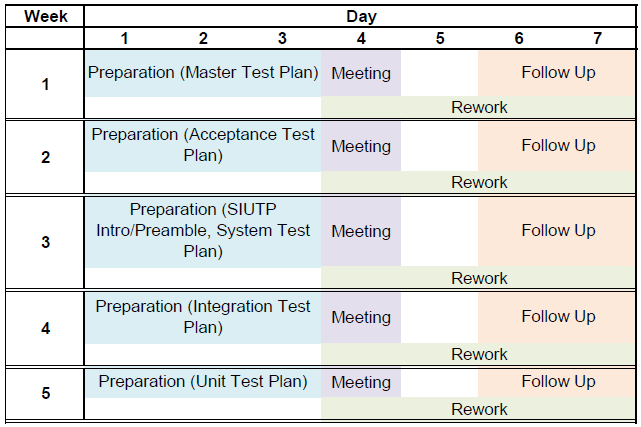
\includegraphics[width=0.8\linewidth]{figures/TP_Schedule.png}
\end{figure}

\clearpage

\subsection{Requirements Verification}\label{sec:srsVV}
The goal of requirements verification is to evaluate the Software Requirements
Specification (SRS) for correctness, consistency, completeness, readability,
testability, and traceability. This corresponds to the requirements evaluation
and traceability analysis tasks in Section 9.2 of IEEE Std
1012-2016~\citep{vvIEEE}.

\paragraph{Method} The SRS verification plan relies on peer review/document
inspection with the following stages:
\begin{enumerate}

    \item Preparation: Participants review the SRS document with respect to
    their assigned role and goals (Table~\ref{tab:rolesSRS})

    \item Meeting: Participants meet to discuss findings, potential issues, and
    proposed action plans to address them

    \item Rework: The SRS author(s) revise the document to address raised
    issues, guided by the proposed action plans

    \item Follow Up: Participants verify that raised issues have been addressed
    satisfactorily

\end{enumerate}

A recording device might be used to capture meeting proceedings in place of
physical note taking so that all participants can focus on the discussion.

Peer review/inspection begins when there is a new major version of the SRS
document.

Peer review/inspection ends when reviewers agree that there are no issues that
will likely result in an extensive loss of confidence in \progname{} (e.g.
barrier to adoption by primary stakeholders).

\paragraph{Roles and Responsibilities} To assist in the achievement of their
assigned goals (Table~\ref{tab:rolesSRS}) using peer review/document inspection:
\begin{itemize}

    \item Primary team members are responsible for ensuring that reviewers have
    the necessary materials, moderating the inspection process and reading
    through the SRS document during the meeting(s)

    \item Secondary and tertiary members are reviewers whom are responsible for
    reviewing the SRS document prior to the meeting(s) so that they are prepared
    to discuss it with the team

\end{itemize}

\paragraph{Inputs}
\begin{itemize}

    \item Software Requirements Specification for \progname{}: A Computational
    Model of Emotion for Enhancing Non-Player Character Believability in Games

    \item Concept Summary for \progname{}: A Computational Model of Emotion for
    Enhancing Non-Player Character Believability in Games

    \item References used to generate primary stakeholder requirements

    \item Review guide for \progname{}'s SRS
    (Appendix~\ref{appendix:srsInspection})

\end{itemize}

\paragraph{Outputs}
\begin{itemize}

    \item Objective evidence to assess the verification of the SRS

    \item Objective evidence that the requirements are complete, correct,
    accurate, and testable

    \item Objective evidence that the requirements are traceable to
    \progname{}'s concept summary and intended use and user needs

    \item Objective evidence that the SRS is readable

    \item Input to Master Test Report (MTR)

\end{itemize}

\paragraph{Estimated Completion Time} Four (4) weeks

Due to the document's size, SRS peer review/inspection is divided into parts.
Only one part is tested per week to reduce participant fatigue:
\begin{itemize}

    \item Part 1: Introduction (Section~2), General System Description
    (Section~3)

    \item Part 2: Problem Description (Section~4.1), Solution Characteristics
    Specification: Emotion Theories and Models (Section~4.2.1), Assumptions
    (Section~4.2.2), Conceptual Models (Section~4.2.3), Theoretical Models
    (Section~4.2.4)

    \item Part 3: Solution Characteristics Specification: General Definitions
    (Section~4.2.5), Data Definitions (Section~4.2.6), Type Definitions
    (Section~4.2.7), Instance Models (Section~4.2.8), Data Constraints
    (Section~4.2.9), Properties of a Correct Solution (Section~4.2.10)

    \item Part 4: Requirements (Section~5), Future Changes (Section~6),
    Traceability Matrices and Graphs (Section~7)

\end{itemize}

\begin{figure}[!h]
    \centering
    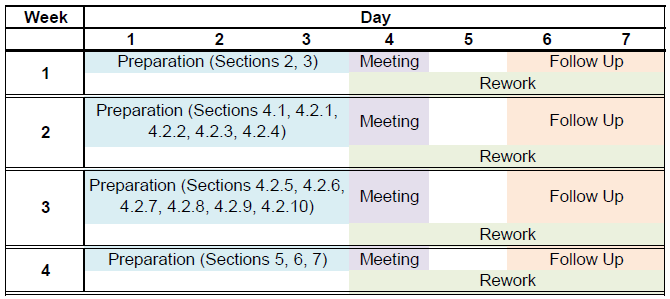
\includegraphics[width=0.9\linewidth]{figures/Requirements_Schedule.png}
\end{figure}

\clearpage

\section{Module Composition into Components and Architecture}
Module decomposition reduced \progname{}'s models into atomic units contained
in ``virtual'' modules that are not implemented (Levels 1 and 2 in
Table~\ref{TblMH}) but this is not necessarily how a user would visualize their
groupings. For example, the hierarchy does not group the Emotion Generation and
Emotion Intensity Function modules together despite their common dependencies
(Figure~\ref{FigUH}). A user might similarly view them as a single unit because
emotion intensity is only relevant if the associated emotion is present.
Therefore, \progname{}'s assignment of the 16 modules to eight components aims
to collect highly-related functionality into a comprehensive unit
(Figure~\ref{fig:components}) that can be exchanged for another with comparable
abilities while reducing inter-component connections
(Figure~\ref{fig:componentConnections}):
\begin{description}

    \item [\refstepcounter{cpnum} \mthecpnum \label{cpIntensity}:] Emotion
    Intensity collects the Emotion Intensity Type (\textbf{\mref{mIntensity}})
    and dependant Emotion State Type (\textbf{\mref{mStateType}}) modules
    because they represent \progname{}'s core emotion types. This also collects
    all \progname{}-specific models necessary for users to define custom
    emotion kinds (\rref{R_MixingEmotionsPES}, \rref{R_PartitionEmotions},
    \rref{R_MixingEmotionsCTE}). Since Emotion Intensity Type does not depend
    on other modules, this only reduces visible dependencies by one because the
    component hides Emotion State Type's dependency on Emotion Intensity Type.

    \item [\refstepcounter{cpnum} \mthecpnum \label{cpGenerate}:] Emotion
    Evaluation collects the Emotion Generation (\textbf{\mref{mGenerate}}) and
    Emotion Intensity Function (\textbf{\mref{mIntensityFun}}) modules due to
    the previously described interdependence of emotion generation and
    intensity calculations. Since these two modules require all the same
    inputs, grouping them as one unit also halves the visible dependencies on
    other modules.

    \item [\refstepcounter{cpnum} \mthecpnum \label{cpDecay}:] Emotion Decay
    collects the Emotion Intensity Decay (\textbf{\mref{mDecay}}) and Emotion
    State Decay (\textbf{\mref{mDecayState}}) because they capture the single
    ``decay emotion'' task. This hides Emotion State Decay's dependency on
    Emotion Intensity Decay while also halving the visible dependencies on other
    modules.

    \item [\refstepcounter{cpnum} \mthecpnum \label{cpEmotion}:] Emotion
    collects the Emotion Type (\textbf{\mref{mEmotionType}}) and Emotion
    Function (\textbf{\mref{mEmotionFun}}) modules because \progname{} intends
    the latter to be helper functions that make Emotion Type easier to use,
    effectively making Emotion Function wholly dependant on Emotion Type. This
    hides Emotion Function's dependency on Emotion Type while also halving the
    visible dependencies on other modules.

    \item [\refstepcounter{cpnum} \mthecpnum \label{cpPAD}:] PAD collects the
    PAD Type (\textbf{\mref{mPADType}}) and PAD Function
    (\textbf{\mref{mPADFun}}) modules because \progname{} only requires a PAD
    data type to contain an emotion state that the PAD Function module has
    transformed into a PAD point. Since PAD Type does not depend on other
    modules, this only reduces visible dependencies by one as the component
    hides PAD Function's dependency on PAD Type.

    \item [\refstepcounter{cpnum} \mthecpnum \label{cpTime}:] Time contains
    only the Time (\textbf{\mref{mTime}}) module. It is separated from the
    World State module (\textbf{\mref{mWorld}}) because there are significantly
    more dependencies on Time than World State, including ones that are
    otherwise independent of the world such as Emotion Decay
    (\textbf{\mref{mDecay}} and \textbf{\mref{mDecayState}}). Time does not
    depend on other modules, so there are no visible dependency reductions.

    \item [\refstepcounter{cpnum} \mthecpnum \label{cpWorld}:] World State
    contains only the World State (\textbf{\mref{mWorld}}) module due to the
    need for Time to be its own component. World State does not depend on other
    modules, so there are no visible dependency reductions.

    \item [\refstepcounter{cpnum} \mthecpnum \label{cpEntity}:] Entity contains
    the Goal (\textbf{\mref{mGoal}}), Plan (\textbf{\mref{mPlan}}), Social
    Attachment (\textbf{\mref{mSocial}}), and Attention
    (\textbf{\mref{mAttention}}) modules because of their common ``entity
    representation'' task. Unlike Time (\textbf{\mref{mTime}}) and World State
    (\textbf{\mref{mWorld}}), there is no need to separate them into different
    components due to a higher number of dependencies on one module and not the
    others. They are also all relied on by the Emotion Evaluation component
    (\textbf{C2}), so collecting the Entity modules together makes its use more
    convenient. There are no dependencies between Goal, Plan, Attention, or
    Social Attachment, so the component does not hide visible dependencies
    within itself. However, Goal and Plan's mutual dependency on World State
    (\textbf{\mref{mWorld}}) is visible as a single connection rather than two
    separate ones.

\end{description}

\vspace*{\fill}
\begin{figure}[!ht]
    \centering
    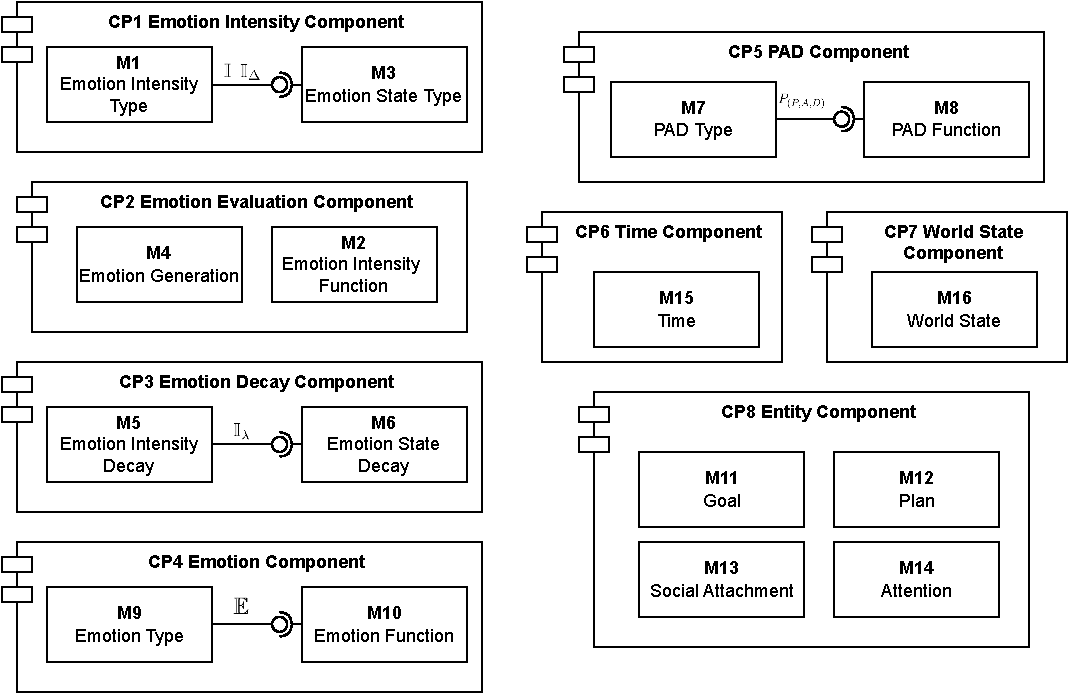
\includegraphics[width=\linewidth]{figures/emgineArch_internalComponents.pdf}
    \caption{Organization of Modules in Components (``Ball'' provides
    functionality that a ``Cup'' needs)}
    \label{fig:components}
\end{figure}
\vspace*{\fill}

\begin{figure}[!ht]
    \centering
    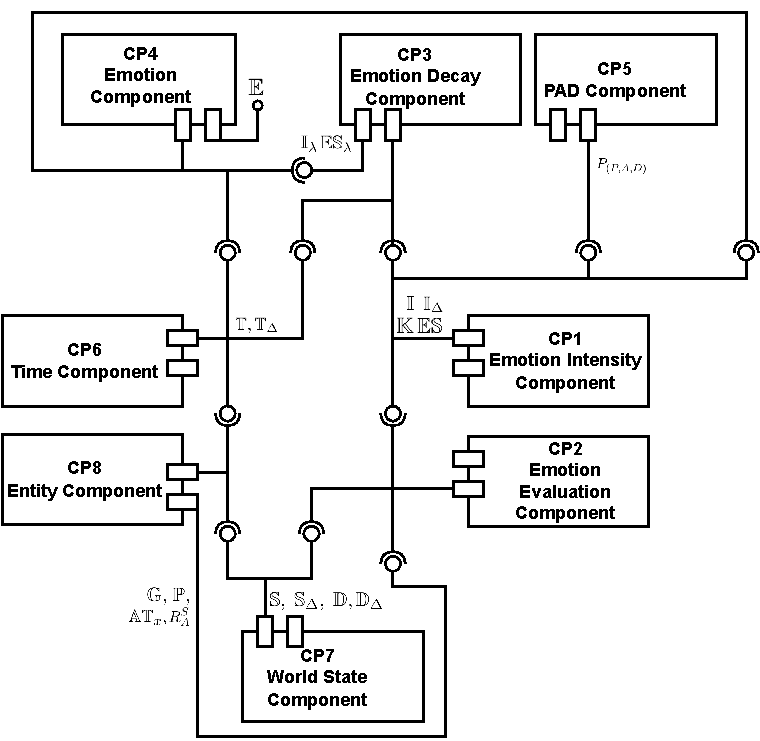
\includegraphics[width=0.7\linewidth]{figures/emgineArch_componentRelations.pdf}
    \caption{Relationships Between Modules (``Ball'' provides functionality
    that a ``Cup'' needs)}
    \label{fig:componentConnections}
\end{figure}

\clearpage

\subsection{Design Definition Verification}\label{sec:designVV}
The goal of design definition verification is to evaluate \progname{}'s
Module Interface Specification (MIS) for correctness, consistency,
completeness, readability, testability, and traceability. This corresponds to
the design evaluation and traceability analysis tasks in Section 9.3 of IEEE
Std 1012-2016~\citep{vvIEEE}.

\paragraph{Method} The MIS verification plan relies on peer review/document
inspection with the following stages:
\begin{enumerate}

    \item Preparation: Participants review the MIS document with respect to
    their assigned role and goals (Table~\ref{tab:rolesMIS})

    \item Meeting: Participants meet to discuss findings, potential issues,
    and proposed action plans to address them

    \item Rework: The MIS author revises the document to address raised issues,
    guided by the proposed action plans

    \item Follow Up: Participants verify that raised issues have been addressed
    satisfactorily

\end{enumerate}

A recording device might be used to capture meeting proceedings in place of
physical note taking so that all participants can focus on the discussion.

Peer review/inspection begins when there is a new major version of the MIS
document.

Peer review/inspection ends when reviewers agree that there are no issues that
will likely result in an extensive loss of confidence in \progname{} (e.g.
insufficient information hiding).

\paragraph{Roles and Responsibilities} To assist in the achievement of their
assigned goals (Table~\ref{tab:rolesMIS}) using peer review/document inspection:
\begin{itemize}

    \item Primary team members are responsible for ensuring that reviewers have
    the necessary materials, moderating the inspection process and reading
    through the document(s) during the meeting(s)

    \item Secondary and tertiary members are reviewers whom are responsible for
    reviewing the MIS document prior to the meeting so that they are prepared to
    discuss it with the team

\end{itemize}

\paragraph{Inputs}
\begin{itemize}

    \item Module Interface Specification for \progname{}: A Computational Model
    of Emotion for Enhancing Non-Player Character Believability in Games

    \item Module Guide for \progname{}: A Computational Model of Emotion for
    Enhancing Non-Player Character Believability in Games

    \item Review guide for \progname{}'s MIS
    (Appendix~\ref{appendix:designInspection})

\end{itemize}

\paragraph{Outputs}
\begin{itemize}

    \item Objective evidence to assess the verification of the MIS

    \item Objective evidence that the module design specifications are
    complete, correct, accurate, and testable

    \item Objective evidence that no unintended features were introduced into
    the design

    \item Objective evidence that the module design specifications represents a
    complete transformation of the requirements described in \progname{}'s
    Software Requirements Specification (SRS)

    \item Objective evidence that the MIS is readable

    \item Input to Master Test Report (MTR)

\end{itemize}

\paragraph{Estimated Completion Time} Four (4) weeks

Due to the number and relative complexity of the modules, MIS verification is
divided into parts by level in the use hierarchy. This ensures that modules are
verified before those that use them so that any necessary changes are made
before their verification. Only one part is tested per week to reduce
participant fatigue:
\begin{itemize}

    \item Part 1: Emotion Intensity Type (M1), Emotion Intensity Decay Rate
    Type (M5), PAD Type (M8), Social Attachment (M15), Time (M16) World State
    (M17)

    \item Part 2: Emotion State Type (M3), Goal (M12), Plan (M13), Attention
    (M14)

    \item Part 3: Emotion Intensity Decay State (M6), Emotion Decay Function
    (M7), PAD Function (M9), Emotion Type (M10)

    \item Part 4: Emotion Intensity Function (M2), Emotion Generation Function
    (M4), Emotion Function (M11)

\end{itemize}

\begin{figure}[!h]
    \centering
    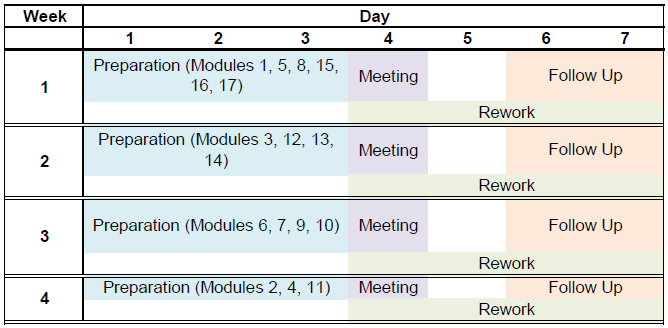
\includegraphics[width=0.9\linewidth]{figures/DesignDef_Schedule.png}
\end{figure}

\clearpage

\subsection{Implementation Verification}\label{plan:implementation}
The goal of implementation verification is to evaluate \progname{}'s source
code and its documentation for correctness, consistency, completeness,
accuracy, readability, testability, and traceability. This corresponds to the
source code and source code documentation evaluation and traceability analysis
tasks in Section 9.4 of IEEE Std 1012-2016~\citep{vvIEEE}.

\paragraph{Method} The implementation verification plan uses both static and
dynamic testing methods:
\begin{enumerate}

    \item Static Testing Method \\
    The source code and its documentation is statically tested by peer review.
    A peer review tests: the source code for traceability to Module Interface
    Specification (MIS) document and consistent use of coding standards and
    quality; and the source code's documentation for correctness, completeness,
    consistency, and readability.

    The peer review has the following stages:
    \begin{enumerate}

        \item Preparation: Participants review the source code and its
        documentation with respect to their assigned role and goals
        (Table~\ref{tab:rolesImplementation})

        \item Meeting: Participants meet to discuss findings, potential issues,
        and proposed action plans to address them

        \item Rework: The source code/documentation author revises the
        code/documentation to address raised issues, guided by the proposed
        action plans

        \item Follow Up: Participants verify that raised issues have been
        addressed satisfactorily

    \end{enumerate}

    A recording device might be used to capture meeting proceedings in place of
    physical note taking so that all participants can focus on the discussion.

    Peer review begins when there is a new major version of the source code
    and/or its documentation.

    Peer review ends when reviewers agree that there are no issues that will
    likely result in an extensive loss of confidence in \progname{} (e.g.
    inconsistent naming conventions).

    \item Dynamic Testing Method \\
    Test cases dynamically test the source code for its adherence to the
    behaviours specified in the functional requirements in the Software
    Requirements Specification (SRS) and the characteristics and/or properties
    specified in the nonfunctional requirements in the SRS.

    For information about test case types, specifications, and traceability to
    \progname{}'s requirements, see the ``System, Integration, and Unit Test
    Plan for \progname{}: A Computational Model of Emotion for Enhancing
    Non-Player Character Believability in Games'' document.

\end{enumerate}

%Dynamic methods:
%\begin{itemize}
%
%    \item Boundary testing
%
%    \item Default/Null testing
%
%    \item Garbage data testing
%
%    \item State testing
%
%    \item Race condition testing
%
%    \item Repetition, Stress, and Load testing
%
%    \item Code coverage testing
%
%\end{itemize}

\paragraph{Roles and Responsibilities} To assist in the achievement of their
assigned goals (Table~\ref{tab:rolesImplementation}):
\begin{enumerate}

    \item Static Testing
    \begin{itemize}

        \item Primary team members are responsible for ensuring that reviewers
        have the necessary materials, moderating the peer review process and
        reading through the document(s) during the meeting(s)

        \item Secondary and tertiary members are reviewers whom are responsible
        for reviewing the source code and source code documentation prior to
        the meeting so that they are prepared to discuss it with the team

    \end{itemize}

    \item Dynamic Testing
    \begin{itemize}

        \item Primary team members are responsible for generating and
        implementing test cases and automated tools as described in the
        ``System, Integration, and Unit Test Plan for \progname{}: A
        Computational Model of Emotion for Enhancing Non-Player Character
        Believability in Games'' document

        \item Secondary and tertiary members do not participate in dynamic
        testing

    \end{itemize}

\end{enumerate}

\paragraph{Inputs}
\begin{itemize}

    \item Source Code and Documentation for \progname{}: A Computational Model
    of Emotion for Enhancing Non-Player Character Believability in Games

    \item Module Guide for \progname{}: A Computational Model of Emotion for
    Enhancing Non-Player Character Believability in Games

    \item Module Interface Specification for \progname{}: A Computational Model
    of Emotion for Enhancing Non-Player Character Believability in Games

    \item Coding standards for the source code's implementation language

    \item Review guide for \progname{}'s source code and its documentation
    (Appendix~\ref{appendix:verificationInspection})

    \item System, Integration, and Unit Test Plan for \progname{}: A
    Computational Model of Emotion for Enhancing Non-Player Character
    Believability in Games

\end{itemize}

\paragraph{Outputs}
\begin{itemize}

    \item Objective evidence to assess the verification of the source code and
    its documentation

    \item Objective evidence that the source code and its documentation are
    correct, accurate, and complete

    \item Objective evidence that the source code correctly implements the
    design specification in \progname{}'s Module Guide (MG) and MIS

    \item Objective evidence that the source code and its documentation are
    readable

    \item Input to Master Test Report (MTR)

    \item Input to the System, Integration, and Unit Test Report (SIUTR)

\end{itemize}

\paragraph{Estimated Completion Time} Four (4) weeks

Due to the number and relative complexity of the modules, source and associated
documentation verification is divided into parts by level in the MIS use
hierarchy. This ensures that a piece of code/documentation is verified before
integration testing with other code units. Only one part is tested per week to
reduce participant fatigue:
\begin{itemize}

    \item Part 1: Emotion Intensity Type (M1), Emotion Intensity Decay Rate
    Type (M5), PAD Type (M8), Social Attachment (M15), Time (M16) World State
    (M17)

    \item Part 2: Emotion State Type (M3), Goal (M12), Plan (M13), Attention
    (M14)

    \item Part 3: Emotion Intensity Decay State (M6), Emotion Decay Function
    (M7), PAD Function (M9), Emotion Type (M10)

    \item Part 4: Emotion Intensity Function (M2), Emotion Generation Function
    (M4), Emotion Function (M11)

\end{itemize}

\begin{figure}[!h]
    \centering
    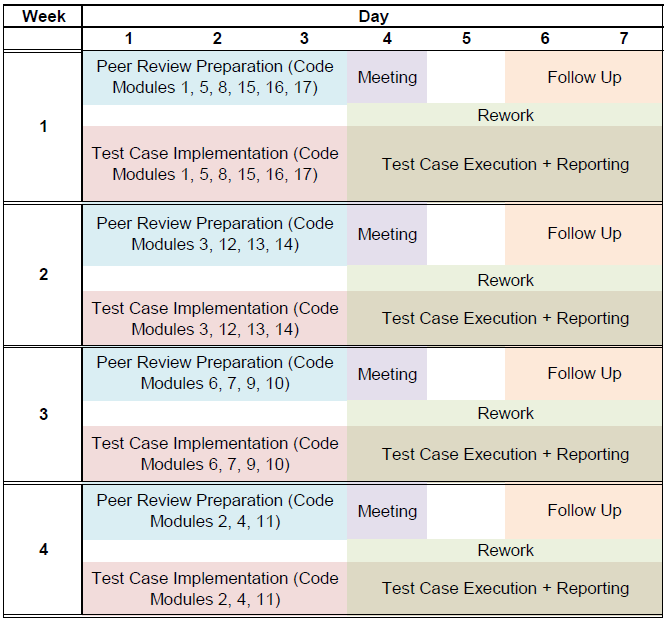
\includegraphics[width=0.9\linewidth]{figures/Implement_Schedule.png}
\end{figure}

\clearpage

\subsection{Implementation Validation}\label{plan:validate}
The goal of implementation validation is to evaluate \progname{}'s ability to
meet its stakeholders' expectations with respect to its behaviour and
characteristics. This corresponds to the software acceptance test procedure V
\& V and traceability analysis tasks in Section 9.7 of IEEE Std
1012-2016~\citep{vvIEEE}.

\paragraph{Method} Validation relies on test cases and user studies:
\begin{itemize}

    \item Test cases evaluate \progname{}'s models to see if they produce the
    ``correct'' emotion type and intensity given an emotion-eliciting context.
    This involves the creation of test cases from scenarios where ``inputs''
    are deducible and ``outputs'' are readily observable.

    \item User studies evaluate meets the needs of \progname{}'s stakeholders
    by involving them directly in the testing process. Their design is based on
    methods and techniques from Human-Computer Interaction (HCI).

\end{itemize}

For information about test case specifications, user study designs, and
traceability to \progname{}'s requirements, see the ``Acceptance Test Plan for
\progname{}: A Computational Model of Emotion for Enhancing Non-Player
Character Believability in Games'' document.

\paragraph{Role Assignments} To assist in the achievement of their
assigned goals (Table~\ref{tab:rolesAcceptance}):
\begin{itemize}

    \item Primary team members are responsible for preparing testing reports
    and providing them to other members of the validation team

    \item Secondary team members are responsible for advising primary members
    during test report preparation in accordance with their expertise

    \item Tertiary team members are responsible for evaluating test reports for
    clarity and comprehensiveness

\end{itemize}

\paragraph{Inputs}
\begin{itemize}

    \item Source Code and Documentation for \progname{}: A Computational Model
    of Emotion for Enhancing Non-Player Character Believability in Games

    \item User Manual for \progname{}: A Computational Model
    of Emotion for Enhancing Non-Player Character Believability in Games

    \item Acceptance Test Plan for \progname{}: A Computational Model of
    Emotion for Enhancing Non-Player Character Believability in Games

    \item Master Test Report (MTR)

    \item System, Integration, and Unit Test Report (SIUTR)

\end{itemize}

\paragraph{Outputs}
\begin{itemize}

    \item Objective evidence that \progname{} satisfies all allocated system
    requirements and its intended use and user needs

    \item Input to MTR

    \item Input to the Acceptance Test Report (ATR)

\end{itemize}

\paragraph{Estimated Completion Time} Two (2) weeks + X $\times$ four (4)
weeks, where X is the number of user studies

This value is derived from estimates pertaining to the quantity of required
test cases and the number and nature of the user studies.

It is difficult to know how many test cases are necessary to validate a CME.
One report estimates that researchers created approximately 600 different
scenarios for a CME with 24 emotion kinds~\citep{elliott1998hunting}. For
\progname{}, this is approximately 200 scenarios for eight emotion kinds.
Accounting for time to analyze and reason about tests the \progname{} fails,
the expected completion time for test case validation is two weeks if roughly
20 test cases are completed per day.

Due to the involvement of human participants, completing user studies is an
extended process. It is estimated that---per user study---data collection will
take approximately two and a half weeks and data analysis one and a half weeks
for a total of four weeks.

    \clearpage

    \section{Test Reporting Requirements}\label{testplan_reporting}
This section describes the type and contents of reports that must be generated
to summarize the results of all Verification and Validation (V \& V) efforts.

\subsection{Master Test Report}\label{reporting:mtr}
The Master Test Report (MTR) provides an overview of all V \& V efforts,
including those documented in other test reports. The document's content and
organization is based on IEEE Std 829-2008 Clause 17: Master Test
Report~\citep{vvDocIEEE}. The MTR must include:
\begin{enumerate}

    \item Document Revision History

    \item Reference Material (e.g. symbols, acronyms, definitions)

    \item Introduction \\
    Identify who prepared the report, its purpose, and its current status (e.g.
    Draft, Final)
    \begin{enumerate}

        \item Scope \\
        Summarize the components of \progname{} tested, which might include a
        reference/addition/ changes to the Master Test Plan (MTP) and/or a
        component's testing history

        \item Relevant Documentation \\
        Provide references to documents necessary for compiling the MTR,
        including the: Acceptance Test Report (Section~\ref{reporting:atr}),
        System, Integration, and Unit Test Report
        (Section~\ref{reporting:siutr}), and all other test reports created
        during V \& V; and Software Development Artifacts (SDAs) and standards
        (e.g. IEEE Std 829-2008)

    \end{enumerate}

    \item Details of the MTR \\
    ``This section describes the overview of all aggregate test results,
    rational for any decisions, and the final conclusions and
    recommendations.''~\citep[p.~67]{vvDocIEEE}
    \begin{enumerate}

        \item Overview of Aggregated Test Results \\
        Provide executive-level summaries of testing activities and tasks with
        references to the MTP (i.e. Section~\ref{testplan_highlevel}),
        categorized summaries of resolved and unresolved issues with references
        to reports (Section~\ref{reporting:issues}), summaries of collected
        metrics, and an overall assessment of \progname{}'s quality with
        justification

        \item Decision Rationale \\
        Explain if \progname{} passes or fails its V \& V; if it conditionally
        passes, describe the qualifying restrictions and/or issues that must be
        resolved for \progname{} to pass

        \item Conclusions and Recommendations \\
        Describe the overall evaluation of \progname{}, recommendations and
        circumstances for use, recommendations concerning its readiness for
        release, lessons learned during testing which might include the
        identification of issue categories and/or root cause analysis, and how
        to handle deferred issues

    \end{enumerate}

\end{enumerate}

\clearpage

\subsection{Acceptance Test Report}\label{reporting:atr}
The Acceptance Test Report (ATR) provides an overview of the testing efforts
made towards executing the ``Acceptance Test Plan for \progname{}: A
Computational Model of Emotion for Enhancing Non-Player Character Believability
in Games''. The document's content and organization is a combination of IEEE
Std 829-2008 Clause 15: Level Interim Test Report and 16: Level Test
Report~\citep{vvDocIEEE}. The ATR must include:
\begin{enumerate}

    \item Document Revision History

    \item Reference Material (e.g. symbols, acronyms, definitions)

    \item Introduction \\
    Identify who prepared the report, its purpose, and its current status (e.g.
    Draft, Final)
    \begin{enumerate}

        \item Scope \\
        Describe the contents and organization of the ATR and references to
        information captured by automated tools that are not contained in the
        ATR

        \item Relevant Documentation \\
        Provide references to documents necessary for understanding the ATR,
        including the: Master Test Plan (MTP), Acceptance Test Plan (ATP),
        relevant Issue Reports (Section~\ref{reporting:issues}), and any
        additional relevant V \& V documentation; and Software Development
        Artifacts (SDAs) and standards (e.g. \citet{vvDocIEEE})

    \end{enumerate}

    \item Details of the ATR \\
    Preamble is ``This section provides an overview of the test status and
    results, detailed test results, the status of issues related to these
    testing efforts, and any changes made from the Acceptance Test Plan
    (ATP).''. If all testing is complete, append ``...rationale for all
    decisions, and the final conclusions and recommendations.''
    \begin{enumerate}

        \item Overview of Test Status and Results \\
        Provide a summary of the status of planned tests and results of testing
        efforts with references to the ATP, record the version and components
        of tested SDAs and the impact that the testing environment might have
        had on the results

        \item Detailed Test Results \\
        Provide a summary of the testing activities and events, relevant
        metrics collected, variances of test items from their specifications
        and from tests to their documentation with explanations for the
        variances, and an evaluation of the comprehensiveness of testing
        efforts (e.g. coverage metrics)

        \item Status of Related Issues \\
        Provide a summary of all related issues with references to their
        associated report (Section~\ref{reporting:issues}) with a description
        of their desired and actual status:
        \begin{itemize}
            \item Resolved with a summary of their resolution
            \item Unresolved (``Open'' or ``In Process'' with a progress
            summary)
            \item Deferred with explanations to address them
        \end{itemize}

        \clearpage

        \item Changes From Plans \\
        Provide a summary of test activities that have not yet been executed
        with justification and describe any changes to testing activities such
        as tests that will not be done and tests that must be rerun

        \item Decision Rationale \\
        When all testing activities are complete, Describe any issues
        considered during decision-making and justify the conclusions drawn
        from test results

        \item Conclusions and Recommendations \\
        When all testing activities are complete, describe the overall
        evaluation of each test activity and its limitations, recommendations
        concerning their readiness for use and under what circumstances, and
        lessons learned during testing which might include the identification
        of issue categories and/or root cause analysis

    \end{enumerate}

\end{enumerate}

\clearpage

\subsection{System, Integration, and Unit Test Report}\label{reporting:siutr}
The System, Integration, and Unit Test Report (SIUTR) provides an overview of
the testing efforts made towards executing the ``System, Integration, and Unit
Test Plan for \progname{}: A Computational Model of Emotion for Enhancing
Non-Player Character Believability in Games''. The SIUTR must include all of
the sections described for the Acceptance Test Report (ATR,
Section~\ref{reporting:atr}) and relate its contents to the System,
Integration, and Unit Test Plan (SIUTP) instead of the Acceptance Test Plan
(ATP).

\clearpage

\subsection{Issue Report}\label{reporting:issues}
The Issue Report (IR) is for documenting any event that happens during testing
that must be investigated. The document's content and organization is a
combination of IEEE Std 829-2008 Clause 14: Anomaly Report~\citep{vvDocIEEE}.
The ATR must include:
\begin{enumerate}

    \item Document Revision History

    \item Introduction \\
    Identify who prepared the report, its purpose, and its current status (e.g.
    Draft, Final)
    \begin{enumerate}

        \item Issue Identification Code/Number

        \item Scope \\
        Describe any contextual information necessary for understanding the IR

        \item Relevant Documentation \\
        Provide references to documents necessary for understanding the IR,
        such as a reference to a test plan and/or report

    \end{enumerate}

    \item Details of the IR \\
    ``This section identifies the items contained in the [IR] including its
    status and corrective actions taken.''~\citep[p.~61]{vvDocIEEE}
    \begin{enumerate}

        \item Summary \\
        Provide a summary of the issue

        \item Status of the Issue \\
        State the current status of the issue as one of:
        \begin{itemize}
            \item Open
            \item Assigned
            \item Fixed
            \item Retested with Fix
            \item Resolved
        \end{itemize}

        \item Description of Issue \\
        Provide a description of the issue, sufficient conditions to
        reproduce it, which might include inputs, expected and actual outputs,
        unexpected outcomes, procedure step, environment, attempts to repeat
        the test, and the involved testers and/or observers, and any
        observations and/or activities that could help isolate and correct the
        issue

        \item Context \\
        Identify the version and components of the Software Development
        Artifact (SDA) and/or Software Development Life Cycle (SDLC) stage the
        issue was discovered in; and the associated test level and items with
        their version level involved in the discovery

        \item Date Discovered \\
        Record the date that the issue was first discovered

        \item Impact \\
        If known, describe the breadth and depth of the issue's impact on
        affected SDAs and/or stakeholder needs, and any known workarounds for
        the issue

        \item Description of Corrective Action \\
        Provide a summary of the activities taken to resolve the issue, which
        can include deferral or retirement of duplicate issue

        \item Conclusions and Recommendations \\
        Describe the source/cause of the issue and/or provide recommendations
        for changes to development and/or testing processes to help prevent
        this issue in the future

    \end{enumerate}

\end{enumerate}

    \clearpage

    \bibliographystyle {ACM-Reference-Format}
    \bibliography{../../../refs/references_test,
    ../../../refs/references_gamedesign, ../../../refs/references,
    ../../../refs/references_documentation}

    \clearpage

    \begin{appendix}

    \section{Peer Review/Inspection Guides}
    These documents are intended as guides for reviewers in the peer
    review/inspection of \progname{}'s Software Development Artifacts (SDAs).
    Moderators are responsible for providing the guides to reviewers.

    \subsection{Master Test Plan Inspection Guide}\label{appendix:mtpInspection}
This list is a guide for reviewers in the peer review of the Master Test Plan
(MTP) document (Section~\ref{sec:mtpVV}). The list organizes prompts by MTP
section in the order that they appear in the document. Reviewers are encouraged
to include their own checks to this guide.

\paragraph{Introduction}
\begin{itemize}

    \item Does the introduction describe the purpose of \progname{}'s MTP?

    \item Does the summary of \progname{} describe its intended purpose?

    \item Does the summary of \progname{} list all of its required
    characteristics?

    \item Are \progname{}'s required characteristics consistent with its
    intended purpose?

    \item Are the aspects of \progname{} and its software development artifacts
    (SDA) that are to be tested unambiguous?

    \item Are the aspects of \progname{} and its SDAs that are \textit{not} to
    be tested unambiguous?

    \item Are the testing objectives consistent with \progname{}'s intended
    purpose and characteristics?

    \item Are the objectives achievable?

    \item Is it clear how each plan relates to \progname{}'s Software
    Development Life Cycle (SDLC)?

    \item Does the relevant documentation list all of \progname{}'s
    documentation-based SDAs?

    \item Does the relevant documentation list all standards used to inform the
    MTP?

\end{itemize}

\paragraph{Plan Overview}
\begin{itemize}

    \item Is the list of team members complete?

    \item Are team member descriptions accurate with respect to their
    professional skills and proficiencies?

    \item Are the high-level goals assigned to each team member unambiguous?

    \item Are the high-level goals assigned to each team member consistent with
    their professional skills and proficiencies?

    \item Are the high-level goals assigned to each team member reasonable for
    each software development stage?

    \item Is there a plan for each of \progname{}'s SDAs?

    \item Are the verification methods reasonable for each SDA?

    \item Are the roles assigned to team members reasonable with respect to
    their professional skills, proficiencies, and schedule?

    \item Are the SDAs listed as necessary inputs for each plan unambiguous?

    \item Are the inputs to each verification method sufficient to complete it?

    \item Are the expected outcomes of each plan unambiguous?

    \item Are the outputs of each verification plan reasonable expectations?

    \item Is the expected completion time for each plan reasonable?

\end{itemize}

\paragraph{Readability}
\begin{itemize}

    \item Is the document well structured?

    \item Is the writing clear and cohesive?

    \item Is the writing concise?

    \item Do all abbreviations appear in ``Symbols, Abbreviations and
    Acronyms'' (Section~\ref{sec:refs})?

    \item Is the document free of spelling and grammar errors?

\end{itemize}

    \clearpage

    \subsection{Acceptance Test Plan Inspection
Guide}\label{appendix:validationInspection}
This list is a guide for reviewers in the peer review of the Acceptance Test
Plan (ATP) document (Section~\ref{sec:mtpVV}). The list organizes prompts by
ATP section in the order that they appear in the document. Reviewers are
encouraged to include their own checks to this guide.

\paragraph{Introduction}
\begin{itemize}

    \item Does the introduction describe the purpose of \progname{}'s ATP?

    \item Does the summary of \progname{} match that of Master Test Plan (MTP)?

    \item Are the aspects of \progname{} that are to be tested by the ATP
    unambiguous?

    \item Are the aspects of \progname{} that are \textit{not} to be tested by
    the ATP unambiguous?

    \item Are the testing objectives consistent with the description in the MTP?

    \item Are the objectives achievable?

    \item Is it clear how the ATP impacts \progname{}'s development?

    \item Does the relevant documentation list all \progname{} documentation
    relevant to the ATP?

    \item Does the relevant documentation list all standards used to inform the
    ATP?

\end{itemize}

\paragraph{Test Case Descriptions}
\begin{itemize}

    \item Is the purpose of the test cases unambiguous?

    \item Is the purpose of the test cases traceable to \progname{}'s concept
    summary?

    \item Is the purpose of the test cases traceable to \progname{}'s users and
    user needs?

    \item Are the inputs to each test case specific?

    \item Are the expected outputs of each test case explicitly defined?

    \item Is the purpose of each test case unambiguous?

    \item Are the methods for quantifying errors unambiguous?

    \item Are the methods for measuring qualitative data unambiguous?

    \item Are the test cases traceable to \progname{}'s concept summary?

    \item Are the test cases traceable to \progname{}'s users and user needs?

    \item Do the number and type of test cases seem sufficient?

\end{itemize}

\paragraph{User Study Descriptions}
\begin{itemize}

    \item Is the purpose of the user study unambiguous?

    \item Is the purpose of the user study traceable to \progname{}'s concept
    summary?

    \item Is the purpose of the user study traceable to \progname{}'s users and
    user needs?

    \item Are descriptions of the anticipated number and type of study
    participants unambiguous?

    \item Are the descriptions of study apparatuses complete?

    \item Are the descriptions of study apparatuses unambiguous?

    \item Are the descriptions of study procedures complete?

    \item Are the descriptions of study procedures unambiguous?

    \item Are the descriptions of independent variables complete?

    \item Are the descriptions of independent variables unambiguous?

    \item Are the descriptions of dependent variables complete?

    \item Are the descriptions of dependent variables unambiguous?

    \item Are descriptions of anticipated control, random, and confounding
    variables unambiguous?

    \item Is the user study replicable?

    \item Do the number and type of user studies seem sufficient?

\end{itemize}

    \clearpage

    \subsection{System, Integration, and Unit Test Plan Inspection
Guide}\label{appendix:siutpInspection}
This list is a guide for reviewers in the peer review of the System,
Integration, and Unit Test Plan (SIUTP) document (Section~\ref{sec:mtpVV}). The
list organizes prompts by SIUTP section in the order that they appear in the
document. Reviewers are encouraged to include their own checks to this guide.

\paragraph{Introduction}
\begin{itemize}

    \item Does the introduction describe the purpose of \progname{}'s SIUTP?

    \item Does the summary of \progname{} match that of Master Test Plan (MTP)?

    \item Are the aspects of \progname{} that are to be tested by the SIUTP
    unambiguous?

    \item Are the aspects of \progname{} that are \textit{not} to be tested by
    the SIUTP unambiguous?

    \item Are the testing objectives consistent with the description in the MTP?

    \item Are the objectives achievable?

    \item Is it clear how the SIUTP impacts \progname{}'s development?

    \item Does the relevant documentation list all \progname{} documentation
    relevant to the SIUTP?

    \item Does the relevant documentation list all standards used to inform the
    SIUTP?

    \item Is the list of tools for automated testing and verification complete?

    \item Is the list of tools for automated testing and verification
    unambiguous?

\end{itemize}

\paragraph{System Test Description}
\begin{itemize}

    \item Are the inputs to each test case specific?

    \item Are the expected outputs of each test case explicitly defined?

    \item Is the purpose of each test case unambiguous?

    \item Are the methods for quantifying errors unambiguous?

    \item Are the methods for measuring qualitative data unambiguous?

    \item Are the test cases traceable to \progname{}'s requirements as
    described in the Software Requirements Specification (SRS)?

    \item Do the test cases represent a complete coverage of \progname{}'s
    requirements as described in the SRS? If not, does it explain why?

\end{itemize}

\paragraph{Integration Test Description}
\begin{itemize}

    \item Are the inputs to each test case specific?

    \item Are the expected outputs of each test case explicitly defined?

    \item Is the purpose of each test case unambiguous?

    \item Are the methods for quantifying errors unambiguous?

    \item Are the methods for measuring qualitative data unambiguous?

    \item Are the test cases traceable to the relationships between
    \progname{}'s modules as described in the the Module Guide (MG)?

    \item Do the test cases represent a complete coverage of the relationships
    between \progname{}'s modules as described in MG? If not, does it explain
    why?

\end{itemize}

\paragraph{Unit Test Description}
\begin{itemize}

    \item Are the inputs to each test case specific?

    \item Are the expected outputs of each test case explicitly defined?

    \item Is the purpose of each test case unambiguous?

    \item Are the methods for quantifying errors unambiguous?

    \item Are the methods for measuring qualitative data unambiguous?

    \item Are the test cases traceable to the constants, types, and/or access
    routines in \progname{}'s modules as described in the the Module Interface
    Specification (MIS)?

    \item Do the test cases represent a complete coverage of the constants,
    types, and/or access routines in \progname{}'s modules as described in the
    the MIS? If not, does it explain why?

\end{itemize}

\paragraph{Readability}
\begin{itemize}

    \item Is the document well structured?

    \item Is the writing clear and cohesive?

    \item Is the writing concise?

    \item Do all symbols, abbreviations, and acronyms in the SIUTP appear in
    the Reference Material?

    \item Is the document free of spelling and grammar errors?

\end{itemize}

    \clearpage

    \subsection{SRS Inspection Guide}\label{appendix:srsInspection}
This list is a guide for reviewers in the peer review of the Software
Requirements Specification (SRS) document (Section~\ref{sec:srsVV}). The list
organizes prompts by SRS section in the order that they appear in the document.
Reviewers are encouraged to include their own checks to this guide.

\paragraph{Introduction}
\begin{itemize}

    \item Does the introduction describe the problem domain?

    \item Is the list of stakeholders complete?

    \item Is the description for each stakeholder accurate?

    \item Are the interests of each stakeholder accurate?

    \item Is the document's purpose described unambiguously?

    \item Is the document's purpose described accurately?

    \item Are the characteristics of the intended reader describing the readers
    of the SRS?

    \item Are the characteristics of the intended reader complete?

    \item Is the document accessible to its intended readers?

    \item Does the scope clearly state what \progname{} will do?

    \item Does the scope state clearly what \progname{} will not do?

    \item Is the description of the SRS's document structure accurate?

\end{itemize}

\paragraph{General System Description}
\begin{itemize}

    \item Is the list of entities in the system context clear?

    \item Is the list of entities in the system context complete?

    \item Are the responsibilities for each entity in the system context clear?

    \item Are the responsibilities for each entity in the system context
    complete?

    \item Is the system context diagram accurate?

    \item Are the user characteristics unambiguous?

    \item Are the user characteristics specific?

    \item Are the system constraints accurate?

    \item Are the system constraints complete?

\end{itemize}

\paragraph{Specific System Description: Problem Description}
\begin{itemize}

    \item Is the terminology and definitions list complete?

    \item Is the physical system description complete?

    \item Is the physical system description accurate?

    \item Are the goal statements abstract?

    \item Are the goal statements a refinement of the ``Scope of the
    Requirements'' section and/or stakeholder needs?

    \item Are the goal statements understandable by non-experts of the domain?

\end{itemize}

\paragraph{Specific System Description: Solution Characteristics Description}
\begin{itemize}

    \item Is the choice of affective theories/models traceable to the goal
    statements?

    \item Does each assumption address a single concern?

    \item Are the assumptions traceable to the ``Scope of the Requirements''
    section and/or stakeholder needs?

    \item Is each assumption referenced at least once?

    \item Is the purpose of the Conceptual Models clear?

    \item Are the Theoretical Models refinements of the Conceptual Models?

    \item Is the list of General Definitions complete?

    \item Are derivations of General Definitions clear?

    \item Is the list of Data Definitions complete?

    \item Are derivations of Data Definitions clear?

    \item Are the Type Definitions abstract?

    \item Are the Type Definitions unambiguous?

    \item Are the Type Definitions referenced by at least one other model/type
    definition?

    \item Is it clear which Type Definitions users are responsible for defining?

    \item Are the Instance Models refinements of other models?

    \item Are the Instance Models abstract?

    \item Are the Instance Models clear?

    \item Are there links between each model/type definition and the
    models/type definitions they are referenced by?

    \item Are there links between each model/type definition and the
    models/type definitions they depend on?

    \item Are the Data Constraints complete?

    \item Are the Data Constraints unambiguous?

    \item Are the Properties of a Correct Solution complete?

    \item Are the Properties of a Correct Solution unambiguous?

\end{itemize}

\paragraph{Requirements}
\begin{itemize}

    \item Are the functional requirements abstract?

    \item Are the functional requirements testable?

    \item Are all functional requirements traceable to a stakeholder
    requirement?

    \item Do the nonfunctional requirements have objective fit criteria?

    \item Are the nonfunctional requirement fit criteria testable?

    \item Are all nonfunctional requirements traceable to a stakeholder
    requirement and/or user characteristic?

\end{itemize}

\paragraph{Future Changes}
\begin{itemize}

    \item Are the likely changes traceable to some component of the SRS?

    \item Is it feasible to hide the likely changes in a design?

\end{itemize}

\paragraph{Traceability Matrices and Graphs}
\begin{itemize}

    \item Are all necessary traceability matrices and graphs present?

    \item Are all necessary traceability matrices and graphs accurate?

\end{itemize}

\paragraph{Readability}
\begin{itemize}

    \item Does the document describe the problem domain?

    \item Is the document well structured?

    \item Is the writing clear and cohesive?

    \item Is the writing concise?

    \item Do all symbols, abbreviations, and notation in the SRS appear in the
    Reference Material?

    \item Is the document free of spelling and grammar errors?

\end{itemize}

    \clearpage

    \subsection{Architecture Inspection Guide}\label{appendix:archInspection}
This list is a guide for reviewers in the peer review of the Module Guide (MG)
document (Section~\ref{sec:archVV}). The list organizes prompts by MG section
in the order that they appear in the document. Reviewers are encouraged to
include their own checks to this guide.

\paragraph{Introduction}
\begin{itemize}

    \item Does the introduction summarize the problem domain described in the
    SRS?

    \item Is the document's purpose described unambiguously?

    \item Is the document's purpose described accurately?

    \item Are the characteristics of the intended reader describing the readers
    of the MG?

    \item Are the characteristics of the intended reader complete?

    \item Is the document accessible to its intended readers?

    \item Is the description of the MG's document structure accurate?

\end{itemize}

\paragraph{Anticipated and Unlikely Changes}
\begin{itemize}

    \item Are the likely changes from the SRS associated with at least one
    anticipated change?

    \item Are the unlikely changes justified?

\end{itemize}

\paragraph{Connection Between Requirements and Design}
\begin{itemize}

    \item Is the justification for the proposed architecture unambiguous?

    \item Is the justification for the proposed architecture traceable to
    stakeholder needs as described in the SRS?

    \item Is the justification for the proposed architecture traceable to one
    or more functional and/or nonfunctional requirements from the SRS?

\end{itemize}

\paragraph{Module Hierarchy and Decomposition}
\begin{itemize}

    \item Do the modules satisfy the principle of information hiding?

    \item Is there one secret per module? If not, is it justified?

    \item Are the behaviour-hiding modules related to requirements in the SRS?

    \item Are the software decision modules related to concepts that are not in
    the SRS?

    \item Are the software decision modules necessary to the design?

\end{itemize}

\paragraph{Traceability Matrices}
\begin{itemize}

    \item Is every functional requirement from the SRS satisfied by at least
    one module?

    \item Is every module used to satisfy at least one functional requirement
    from the SRS?

    \item Is there one anticipated change per module? If not, is it justified?

\end{itemize}

\paragraph{Use Hierarchy Between Modules}
\begin{itemize}

    \item Is the use hierarchy complete?

    \item Is the use hierarchy accurate?

    \item Is the use hierarchy hierarchical?

    \item Does the hierarchy satisfy the principle of low coupling between
    modules?

\end{itemize}

\paragraph{Readability}
\begin{itemize}

    \item Is the document well structured?

    \item Is the writing clear and cohesive?

    \item Is the writing concise?

    \item Do all symbols, abbreviations, and notation in the MG appear in the
    Reference Material?

    \item Is the document free of spelling and grammar errors?

\end{itemize}

    \clearpage

    \subsection{Design Inspection Guide}\label{appendix:designInspection}
This list is a guide for reviewers in the peer review of the Module Interface
Specification (MIS) document (Section~\ref{sec:designVV}). The list organizes
prompts by MIS section in the order that they appear in the document. Reviewers
are encouraged to include their own checks to this guide.

\paragraph{Introduction}
\begin{itemize}

    \item Does the introduction summarize the problem domain described in the
    SRS?

    \item Does the introduction have references/links to the SRS and MG?

\end{itemize}

\paragraph{Notation}
\begin{itemize}

    \item Is the notation unambiguous?

    \item Is the notation complete?

    \item Is the notation used consistently throughout the MIS?

\end{itemize}

\paragraph{Module Hierarchy}
\begin{itemize}

    \item Does the module hierarchy match the MG?

    \item Is there a specification for each module in the module hierarchy?

\end{itemize}

\paragraph{Module Specifications}
\begin{itemize}

    \item Does the introductory content describe the purpose and key
    characteristics of the module?

    \item Are the modules classified correctly (e.g. Interface, ADT, Generic)?

    \item Are all exported constants defined with a literal value?

    \item Are the assumptions justified?

    \item Do all access routines do something (i.e. output or state transition)?

    \item Are all operations type safe?

    \item Are all state invariants initially satisfied?

    \item Are all state invariants satisfied when an access routine terminates?

    \item Do local functions make the specification easier to understand?

    \item Does each module satisfy the principle of high cohesion?

\end{itemize}

\paragraph{Readability}
\begin{itemize}

    \item Is the document well structured?

    \item Is the writing clear and cohesive?

    \item Is the writing concise?

    \item Do all symbols, abbreviations, and notation in the MIS appear/have a
    reference to a definition in the Reference Material?

    \item Is the document free of spelling and grammar errors?

\end{itemize}

    \clearpage

    \subsection{Implementation Inspection
Guide}\label{appendix:verificationInspection}
This list is a guide for reviewers in the peer review of the source code and
source code documentation (Section~\ref{plan:implementation}). The list
includes prompts for reviewing test case documentation, source code, and source
code documentation. Reviewers are encouraged to include their own checks to
this guide.

\paragraph{Test Case Documentation}
\begin{itemize}

    \item Is the documentation's purpose described unambiguously?

    \item Is the documentation's purpose described accurately?

    \item Is the scope of the test case verification accurate?

    \item Are the types of test cases used accurate?

    \item Are the types of test cases used sufficient?

    \item Are automated testing and/or verification tools documented?

    \item Do the test cases have specific inputs?

    \item Do the test cases have explicitly defined expected outputs?

    \item Is every functional requirement from the SRS satisfied by at least
    one system-level test case?

    \item Is there at least one test case where a set of modules is tested as
    an integrated unit such that only one new module is added to the set in a
    single test case?

    \item Are there sufficient test cases for each module?

\end{itemize}

\paragraph{Source Code and Documentation}
\begin{itemize}

    \item Does each source code file have a header listing the:
    \begin{itemize}
        \item Last modified date
        \item Programming language and its version
        \item Imported libraries and/or components and their version
        \item Operating System and its version
        \item License
        \item Author(s)
    \end{itemize}

    \item Does each function have a header describing its purpose, inputs, and
    outputs?

    \item Are the coding standards of the implementation language used
    consistently throughout the source code and its documentation?

    \item Are constants named consistently?

    \item Are constants given symbolic names?

    \item Are variables named consistently?

    \item Are functions named consistently?

    \item Are source code files organized consistently with respect to each
    other?

    \item Are source code files formatted consistently with respect to each
    other?

    \item Is the source code as simple as possible?

    \item Are modifications to the source code clearly documented?

    \item Is the source code documentation complete/traceable to the source
    code?

    \item Is the source code documentation unambiguous?

\end{itemize}

\paragraph{Readability}
\begin{itemize}

    \item Is the code/document well structured?

    \item Is the writing clear and cohesive?

    \item Is the writing concise?

    \item (If applicable) Do all symbols, abbreviations, and notation in the
    document appear/have a reference to a definition in the Reference Material?

    \item Is the code/document free of spelling and grammar errors?

\end{itemize}

\end{appendix}

\end{document}